\let\negmedspace\undefined
\let\negthickspace\undefined
\documentclass[journal,12pt,onecolumn]{IEEEtran}
\usepackage{cite}
\usepackage{amsmath,amssymb,amsfonts,amsthm}
\usepackage{algorithmic}
\usepackage{graphicx}
\graphicspath{{./figs/}}
\usepackage{textcomp}
\usepackage{xcolor}
\usepackage{txfonts}
\usepackage{listings}
\usepackage{enumitem}
\usepackage{mathtools}
\usepackage{gensymb}
\usepackage{comment}
\usepackage{caption}
\usepackage[breaklinks=true]{hyperref}
\usepackage{tkz-euclide} 
\usepackage{listings}
\usepackage{gvv}                                        
%\def\inputGnumericTable{}                                 
\usepackage[latin1]{inputenc}     
\usepackage{xparse}
\usepackage{color}                                            
\usepackage{array}
\usepackage{longtable}                                       
\usepackage{calc}                                             
\usepackage{multirow}
\usepackage{multicol}
\usepackage{hhline}                                           
\usepackage{ifthen}                                           
\usepackage{lscape}
\usepackage{tabularx}
\usepackage{array}
\usepackage{float}
\newtheorem{theorem}{Theorem}[section]
\newtheorem{problem}{Problem}
\newtheorem{proposition}{Proposition}[section]
\newtheorem{lemma}{Lemma}[section]
\newtheorem{corollary}[theorem]{Corollary}
\newtheorem{example}{Example}[section]
\newtheorem{definition}[problem]{Definition}
\newcommand{\BEQA}{\begin{eqnarray}}
\newcommand{\EEQA}{\end{eqnarray}}
\newcommand{\define}{\stackrel{\triangle}{=}}
\theoremstyle{remark}
\newtheorem{rem}{Remark}

\begin{document}

\title{4.3.38}
\author{ee25btech11048 - Revanth SIVA Kumar}
\maketitle
\renewcommand{\thefigure}{\theenumi}
\renewcommand{\thetable}{\theenumi}

\textbf{Question :} Solve the system of equations
\[
\begin{aligned}
5x - y + 4z &= 5\\
2x + 3y + 5z &= 2\\
5x - 2y + 6z &= -1
\end{aligned}
\]

\textbf{Solution :}

\begin{table}[h!]
  \centering
  \begin{tabular}{|c|c|}
\hline
\textbf{Name} & \textbf{Value} \\ \hline
$\vec{A}$ & $\myvec{2 & 1 \\0 & 3}$ \\ \hline
\end{tabular}

  \caption*{Table : Equations}
  \label{4.3.38}
\end{table}

The system of equations in matrix form is :

\begin{align}
  \myvec{5 & -1 & 4\\2 & 3 & 5\\5 & -2 & 6}\myvec{x\\y\\z} &= \myvec{5\\2\\-1}
\end{align}

Forming the augmented matrix,

\begin{align}
  \myaugvec{3}{5 & -1 & 4 & 5\\2 & 3 & 5 & 2\\5 & -2 & 6 & -1}
\end{align}

Using Gaussian elimination,

\begin{align}
  \myaugvec{3}{5 & -1 & 4 & 5\\2 & 3 & 5 & 2\\5 & -2 & 6 & -1}
  \xleftrightarrow[\;R_2 \to R_2 - \tfrac{2}{5}R_1\;]{\;R_3 \to R_3 - R_1}
  \myaugvec{3}{5 & -1 & 4 & 5\\0 & \tfrac{17}{5} & \tfrac{17}{5} & 0\\0 & -1 & 2 & -6}
\end{align}

\begin{align}
  \xleftrightarrow{R_3 \to R_3 + \tfrac{5}{17}R_2}
  \myaugvec{3}{5 & -1 & 4 & 5\\0 & \tfrac{17}{5} & \tfrac{17}{5} & 0\\0 & 0 & 3 & -6}
\end{align}

Using back substitution we get :

\begin{align}
  3z &= -6 \\
  z &= -2 \\
  \tfrac{17}{5}y + \tfrac{17}{5}z &= 0 \quad\Rightarrow\quad y+z=0\\
  y &= -z = 2\\
  5x - y + 4z &= 5\\
  5x - 2 + 4(-2) &= 5\\
  5x -10 &= 5\\
  x &= 3
\end{align}

\pagebreak

Therefore the solution for the system of equations is : 

\begin{align}
  \myvec{3\\[0.5em]2\\[0.5em]-2}
\end{align}

\pagebreak

\begin{figure}[h!]
  \centering
  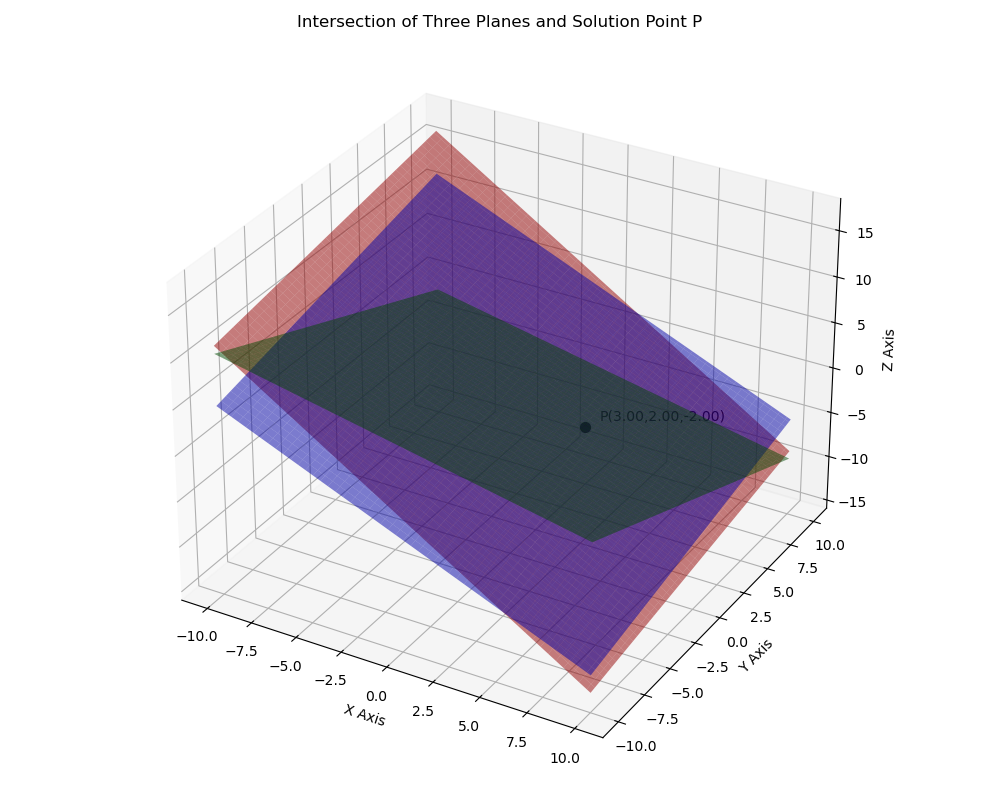
\includegraphics[width=0.9\columnwidth]{figs/Figure_1.png} 
   \caption*{Fig : Planes}
  \label{Fig1}
\end{figure}

\end{document}
